\section{Unsupervised painting detection}
\label{sec:unsupervised_painting_detection}

\subsection{The detection algorithm}
\label{subsec:detection-algo}

The second detection algorithm drastically differs from the first attempt (see \sectionref{subsec:contour_detection}), it was designed from scratch with the weaknesses of the previous algorithm in mind. A little insipiration was taken from Geoff Natin (\cite{natin2020}).

The first step in the algorithm is a mean shift segmentation (see \figureref{fig:paiting_detection_mean_shift})). This is a method to remove noise by taking the mean of the pixels within a certain range. A big advantage is that it partialy removes color gradients and fine-grain textures which would cause issues in the further steps of the algorithm.

\begin{figure}[h]
    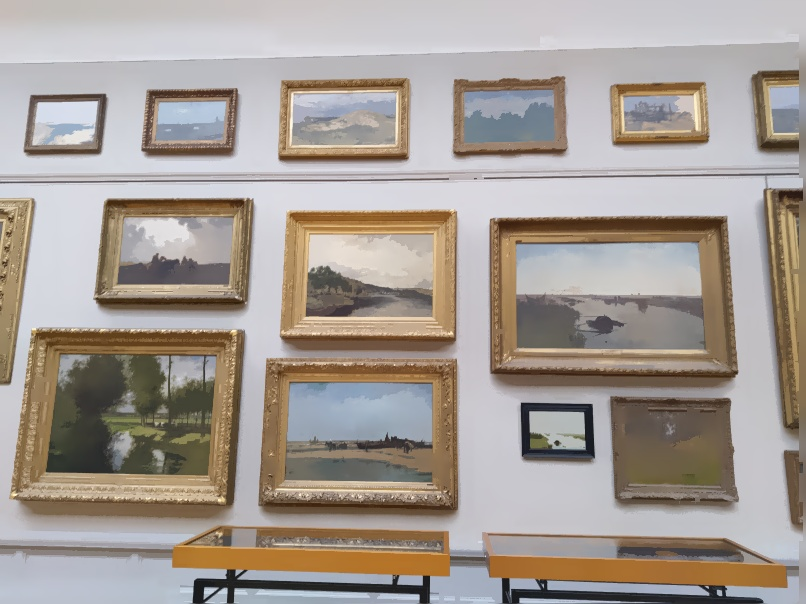
\includegraphics[width=8cm]{IMG_20190323_121447_mean-shift.jpg}
    \centering
    \caption{An example image after mean shift segmentation}
    \label{fig:paiting_detection_mean_shift}
\end{figure}

A common technique in object detection is by creating a mask of the object. The problem with this is that there's no certainty about the size and ratio of the painting as well as where the painting is located in the image and how many there are in the image. This can be solved by thinking the other way around. The one certainty that is consistent throughout all images is that all paintings hang on a wall. A mask for the wall will be made instead of making a mask for the paintings. The mask of the painting(s) can then be obtained by simply inverting this mask.

Another issue is that this mask can't be statically programmed in code for each image since the algorithm needs to be usable on any image or video frame. This can be solved by using a technique called flooding. Flooding will create a mask from a starting position in the image and will fill all neighbouring pixels if they have a color close to the color of the starting position. This is done recursively until no pixels are within the color range of the starting position anymore. \cite{he2019scan}

\begin{figure}[h]
    \centering
    \begin{minipage}[b]{0.45\textwidth}
        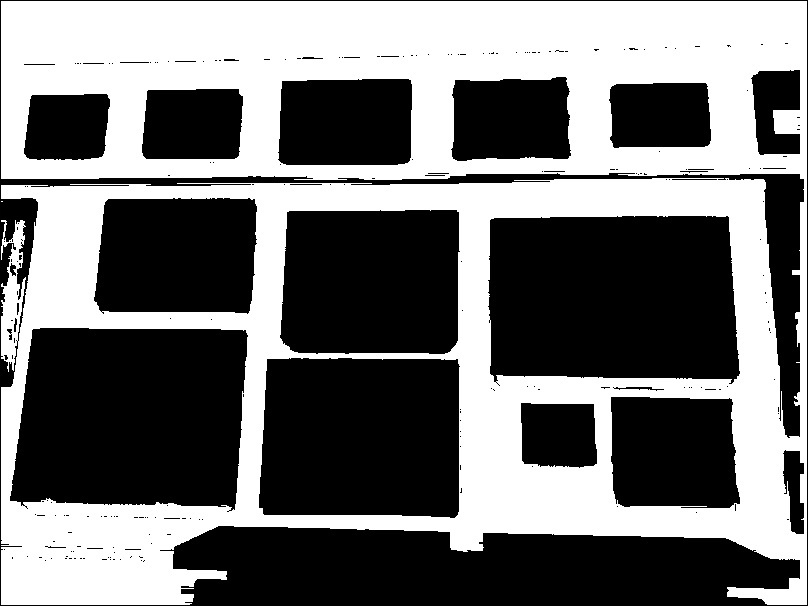
\includegraphics[width=\textwidth]{IMG_20190323_121447_wall-mask.jpg}
        \caption{The wall mask for the example image}
        \label{fig:paiting_detection_wall-mask}
    \end{minipage}
    \hfill
    \begin{minipage}[b]{0.45\textwidth}
        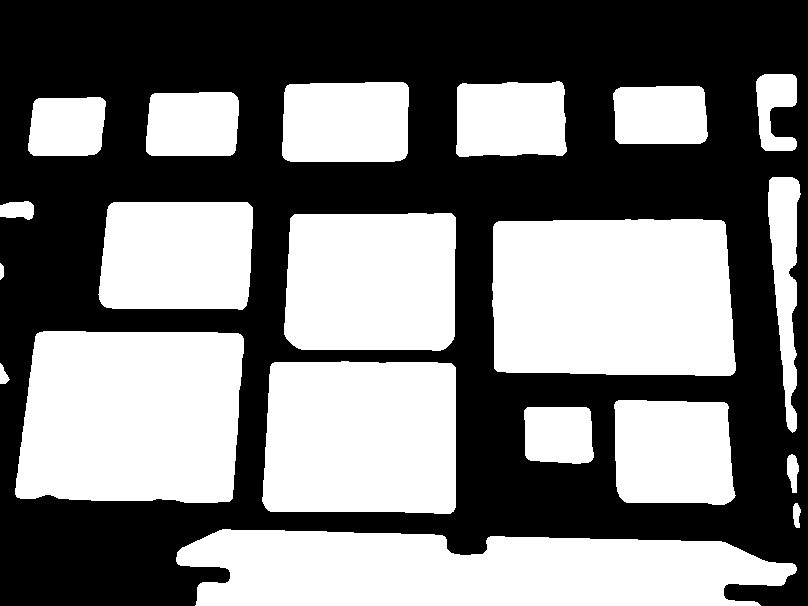
\includegraphics[width=\textwidth]{IMG_20190323_121447_paintings-mask.jpg}
        \caption{The Painting mask for the example image}
        \label{fig:paiting_detection_paintings-mask}
    \end{minipage}
\end{figure}

The next problem is that there needs to be a good starting position to have a good and correct mask for the wall. To find this, the unsupervised algorithm will iterate over all pixels of the image with a certain step size and perform the flooding with that pixel as starting position. Once a mask that has the same height and width as the image is found, then this mask will be used in the next steps of the algorithm. If no such mask is found after iterating over all pixels (with a certain step size), then the mask with the biggest size is used. This is because sometimes parts of the floor or other elements in the image will obstruct the floodfill algorithm to find a mask that has the same size as the image. See \figureref{fig:paiting_detection_wall-mask}) for an example of such mask.

Once the mask of the wall has been obtained, it is inverted to have the mask of the paintings (see \figureref{fig:paiting_detection_paintings-mask}). The mask is then eroded to remove small imperfections and a median blur is used to smooth the edges in the mask.

The next step is to use Canny, the difference with the naive approach is that the two threshold values are determined by using the Otsu algorithm.

Next, a morphological transformations is performed on the Canny edges (see \figureref{fig:paiting_detection_paintings-edges}). This will close edges that are close to each other as this will improve the detection of closed contours. This morphological transformation is in essence a dilation followed by an erosion.

\begin{figure}[ht]
    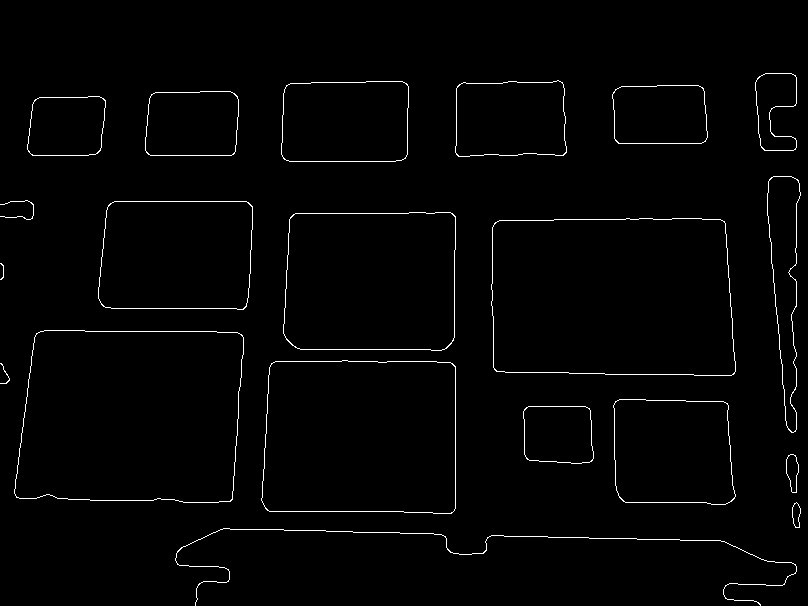
\includegraphics[width=8cm]{IMG_20190323_121447_edges.jpg}
    \centering
    \caption{The edges of the detected paintings}
    \label{fig:paiting_detection_paintings-edges}
\end{figure}

The next steps are exactly the same as the naive painting detection algorithm as described before. The contours are detected in the Canny edges and only fully enclosed polygons with 4 sides are returned as quadrilaterals.

\subsection{Strengths and weaknesses}

The most important improvement of the detection algorithm is that it isn't based on smearing out colors and finding contours in the color smudges.

The key to success with this algorithm is the use of automatic mask creation by using floodfill as main technique. Most of the paintings are detected in most of the images. The detected paintings also have a better fit compared to the naive algorithm.

Most paintings in the dataset are correctly detected as well those in the test set. Only on some occasions there is a miss detection. One flaw that has been found is that some doorways are detected as a paintings. This is logical because of how the mask creation works with the floodfilling. In the case of such a detection flaw, the doorways obstructs the floodfilling algorithm to correctly create a mask of the non-painting area. However, this is something that doesn't happen too often.

A minor problem with this algorithm, which is also the case in the naive algorithm, is that it sometimes detects dark shadows as part of the painting. Although, this is less of an issue in this algorithm then it was in the naive algorithm. It doesn't affect the accuracy too much because if there is a shadow, it only appears on one side of the painting and it doesn't reach far.

A drawback of this algorithm is that it is less performant than the naive algorithm. This is mainly because of the mask creation, specifically the floodfilling. To solve this problem the critical and less performant parts of the algorithm were transformed into Cython. This resolved the whole performance issue and increased the processing performance drastically. \cite{behnel2011cython}

\subsection{Quantitative comparison}
In order to make a quantitative comparison, two things are needed. First of all, the quadrilaterals have to be found autonomously (as described in \sectionref{subsec:contour_detection}). The second thing needed is the groundtruth of the dataset which has been generated by using the solution created with the first algorithm (see \sectionref{sec:assignment1}).

To measure the accuracy of the painting detection algorithm, three things are required; the amount of false negatives (= paintings that aren't found at all), the amount of false positives (= detected paintings that aren't paintings) and the bounding box accuracy (= average intersection divided by union).

With the creation of the solution for this problem, a new problem occured: how to find the intersection of these two shapes? The solution to this problem is made by using ``Shapely''. To do so, the quadrilaterals have to be transformed into a polygon. Once this is done, ``Shapely'' can compute the intersection. It has been tested whether this gives correct intersections if two polygons are not intersecting, or when they are sharing only a line. Also some more general intersections have been tested. Once the intersection is made, it's easy to find the area of the polygon, using ``Shapely'' once again.

The accuracy results for this detection algorithm were fairly good. An example of the detection can be found in \figureref{fig:paiting_detection_with_ground_truth}. The detected contours are shown in red and the groundtruth is shown in blue as determined with the use of the naive algorithm. The dataset consists of 553 images which all together contain 836 paintings. The detection algorithm had 86 false negatives and 32 false positives. The average bounding box accuracy is 81.30\%. These results are displayed on the graphs in \figureref{fig:performance-measurements}.

\begin{figure}[ht]
    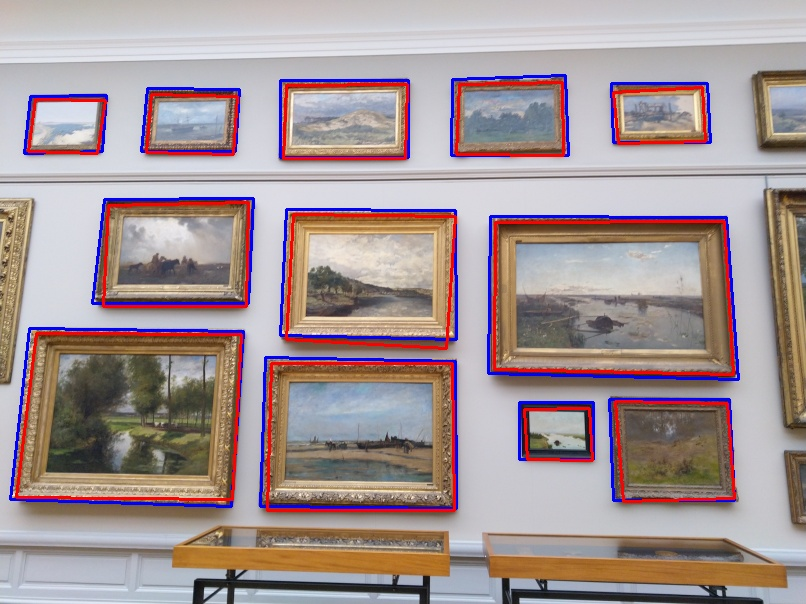
\includegraphics[width=8cm]{IMG_20190323_121447.jpg}
    \centering
    \caption{A visualization of the detected paintings}
    \label{fig:paiting_detection_with_ground_truth}
\end{figure}

\begin{figure}
    \centering
    \begin{tabular}{@{}c@{}}
        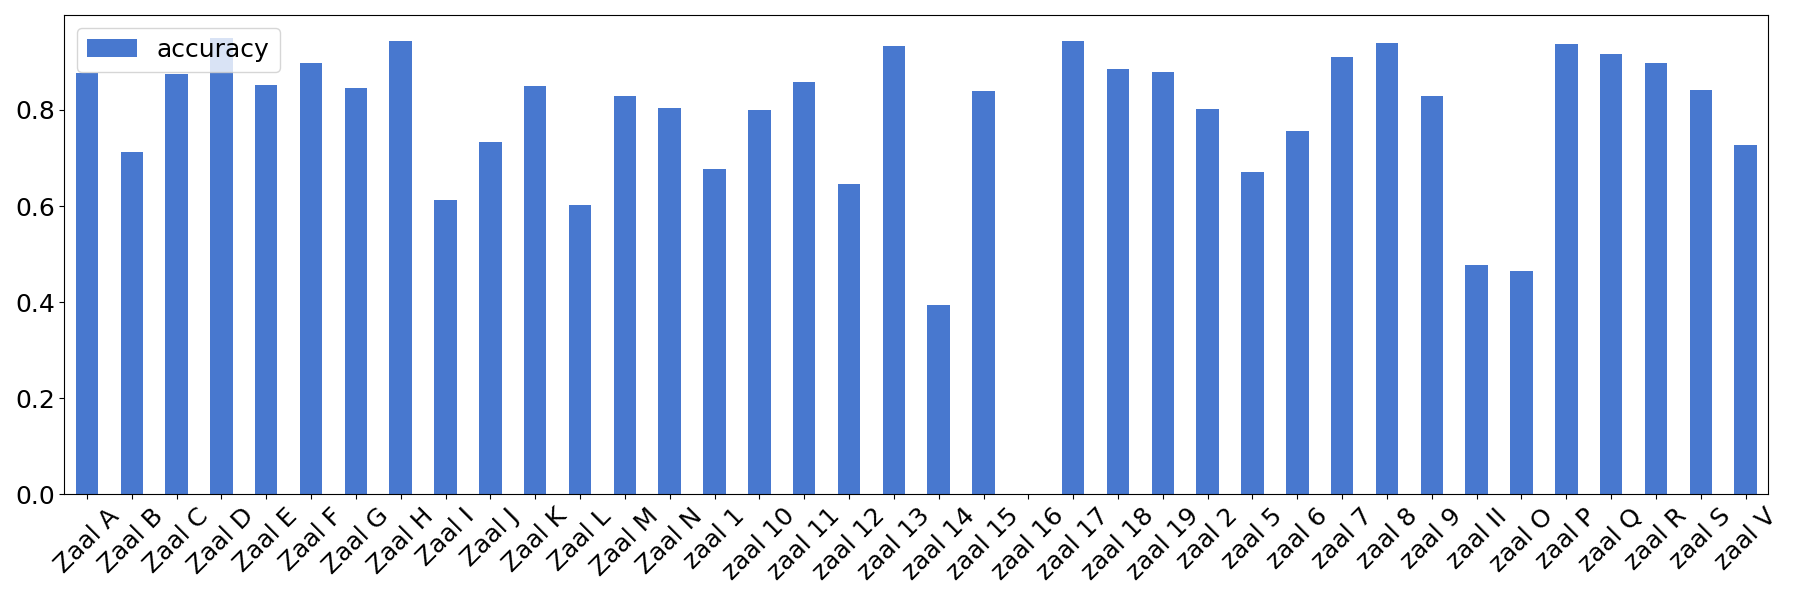
\includegraphics[width=\linewidth]{average_accuracy_per_room.png} \\[\abovecaptionskip]
        \small (a) Average room detection accuracy
    \end{tabular}

    \vspace{\floatsep}

    \begin{tabular}{@{}c@{}}
        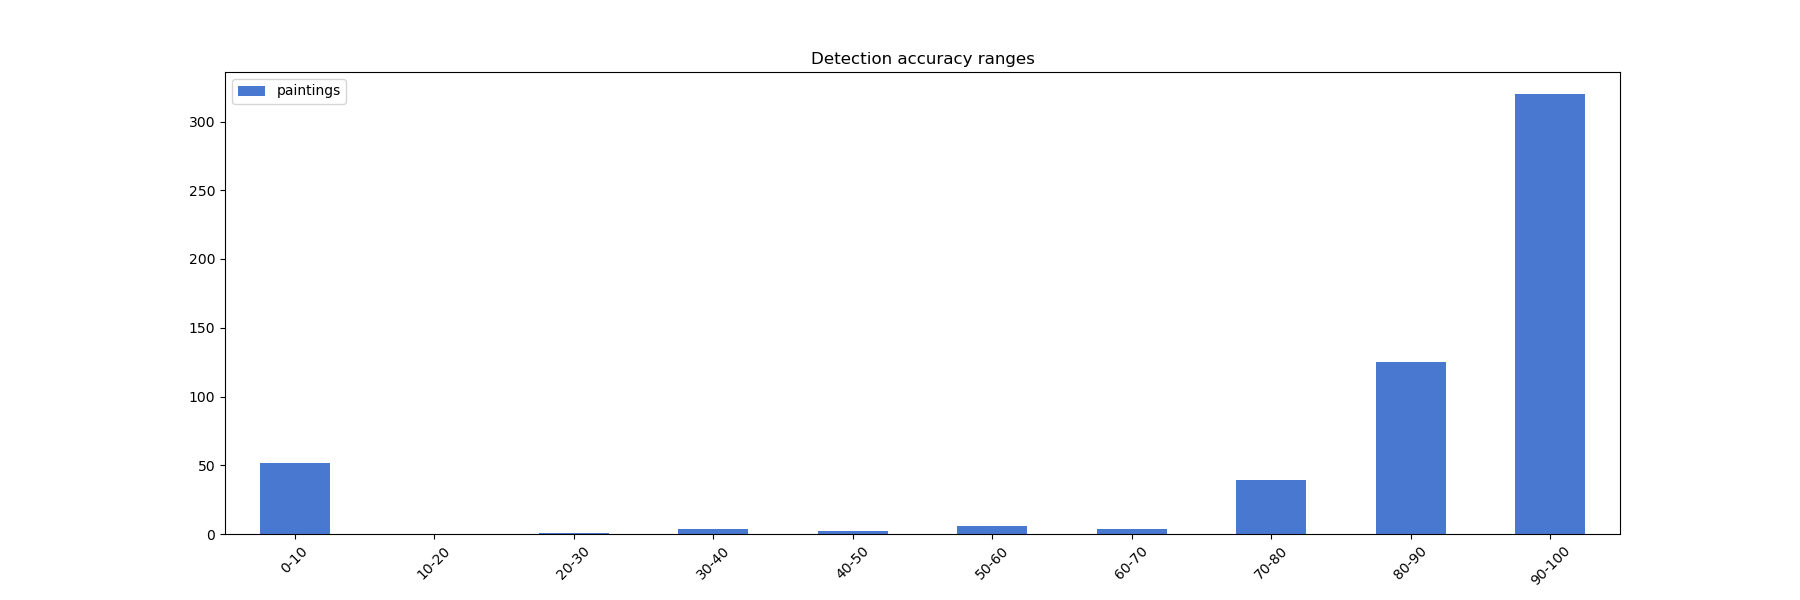
\includegraphics[width=\linewidth]{detection_accuracy_ranges.png} \\[\abovecaptionskip]
        \small (b) Detection accuracy ranges for the dataset
    \end{tabular}

    \begin{tabular}{@{}c@{}}
        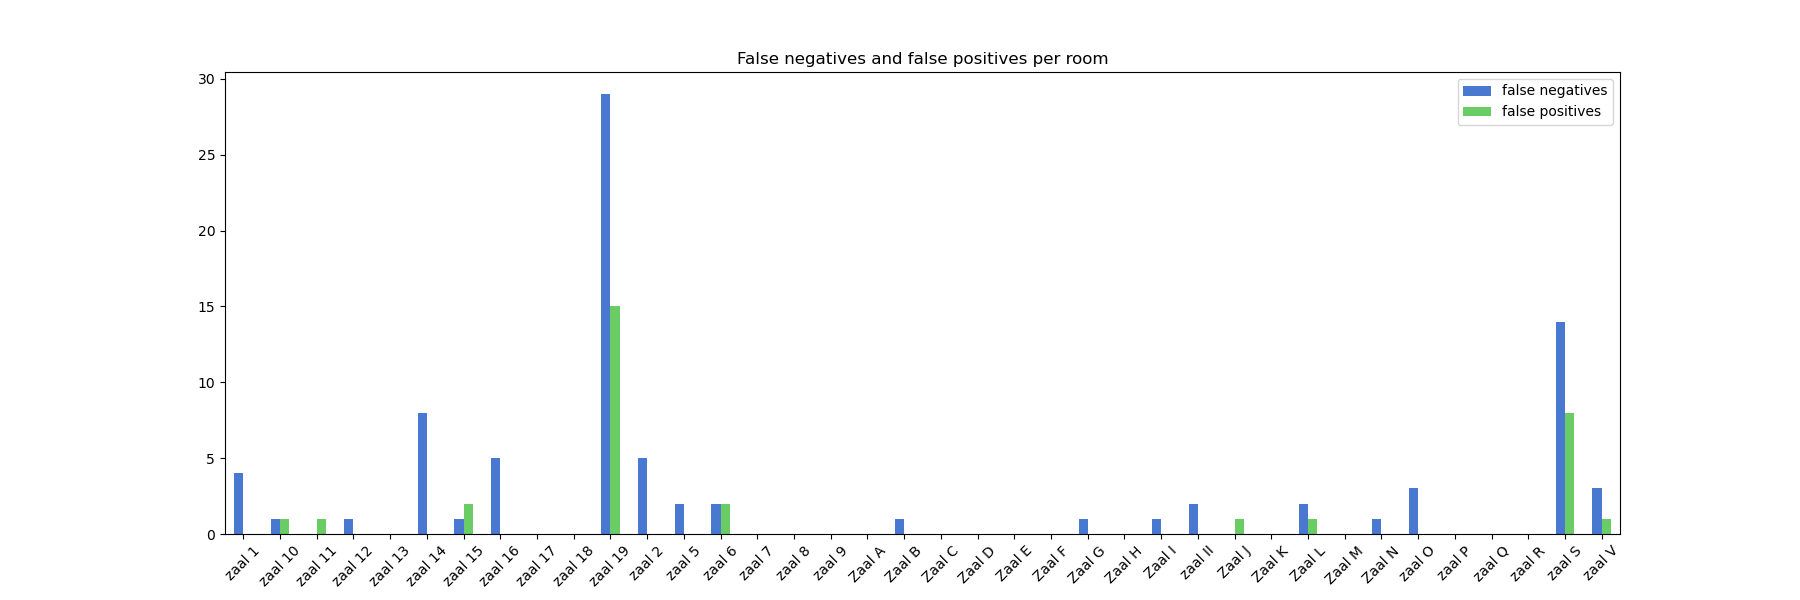
\includegraphics[width=\linewidth]{false_negatives_false_positives.png} \\[\abovecaptionskip]
        \small (c) False negatives and false positives per room
    \end{tabular}

    \caption{Performance measurements}
    \label{fig:performance-measurements}
\end{figure}

\subsection{Qualitative evaluation}
For the qualitative evaluation, the unsupervised painting detection algorithm is used to check how accurate the paintings are found on a more difficult set. Hereby the test set and the video files are used. The painting detection is working well, most paintings are being found. However, some difficulties occur. The algorithm sometimes defines a window as being a painting and it almost always defines a doorway as painting.

Another problem is images shot at a sharp angle. For example when it seems like the borders of two adjacent paintings are overlapping. These images are sometimes not recognized. Paintings in images that are too blurred are sometimes not found either.
